% !TEX root = ../thesis.tex
% developping software for optimization experiments
% @author Tobias Wulf
%

\chapter{Software-Entwicklung für Optimierungsexperimente 0.0.2 19.02.2021}\label{ch:sw-entwicklung-f-opt-exp}

\section{Aufgabe und Funktionen der Software}\label{sec:aufgabe-und-funktionen-sw}
\begin{itemize}
	\item Identifizierung der Grundfunktionen
	\item Datengenerierung
	\item Datenanalyse
	\item Sonderfunktion
	\item Darstellungs- und Plot-Funktionen
\end{itemize}


\begin{figure}[htbp]
	\centering
	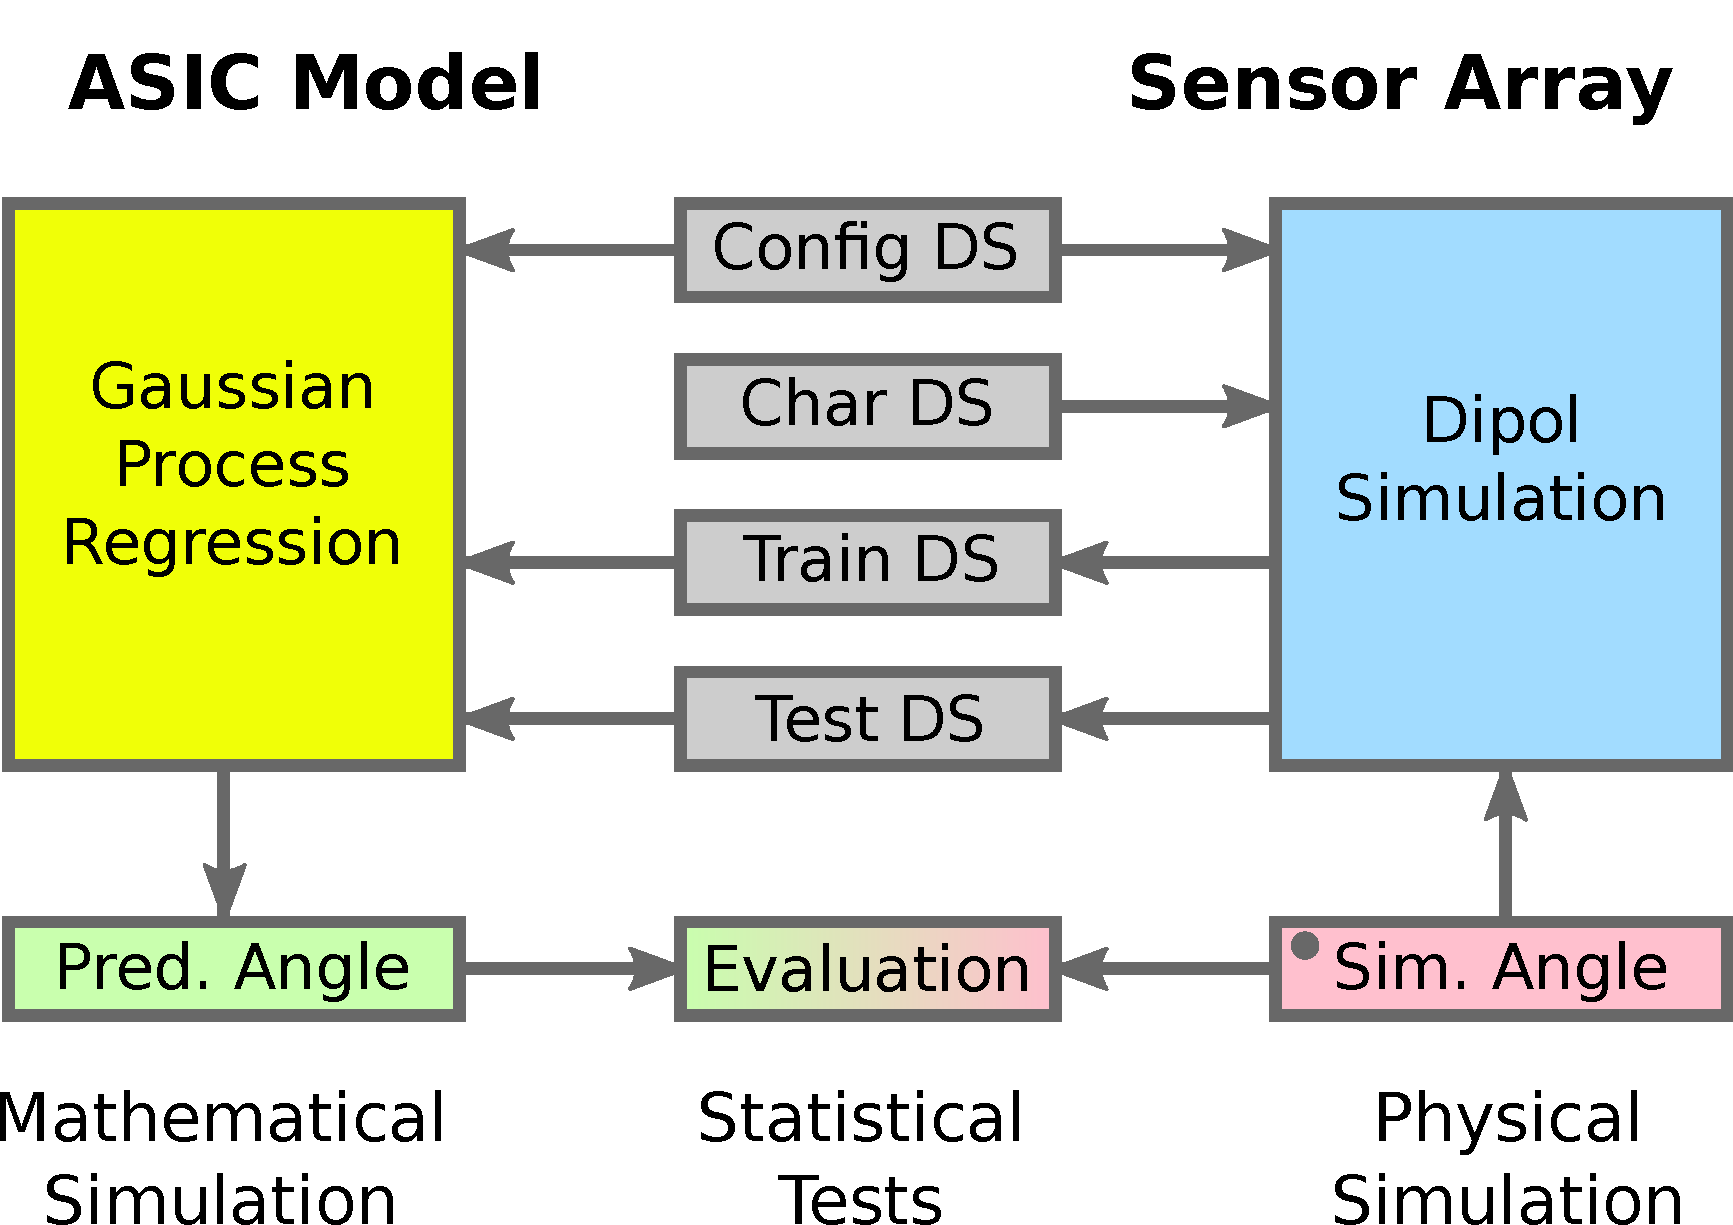
\includegraphics[width=0.7\linewidth]{chapters/images/3-SW-E-OExp/Software-Gesamtansicht}
	\caption[Simulationsaufbau im Überblick]{Simulationsaufbaut im Überblick}
	\label{fig:software-gesamtansicht}
\end{figure}



Die Software-Entwicklung erfolgt unter dem Gesichtspunkt zur Durchführung von Versuchsreihen zu 
Parameterfindung und teilweise auf Zwischenergebnissen basieren.
Gut strukturierte Archivierung von Ergebnisse.
Graphische Unterstützung von Auswertung.
 
\section{Aufbau und Vorgehen}\label{sec:aufbau-und-vorgehen}
	\begin{itemize}
		\item Skriptbasierte Entwurfsarbeit
		\item Überführen in modularen Aufbau von Kernfunktion
		\item Parametrierte Steuerung der Software über Zentrale Konfigurierung
		\item Ausführbare Skripte (Einbindung von Modulen und nutzen der Konfigurierung)
		\item Speicherung von Ergebnissen in Datensätzen
		\item Versionierung der Arbeitsschritte
	\end{itemize}


\begin{figure}[tbph]
	\centering
	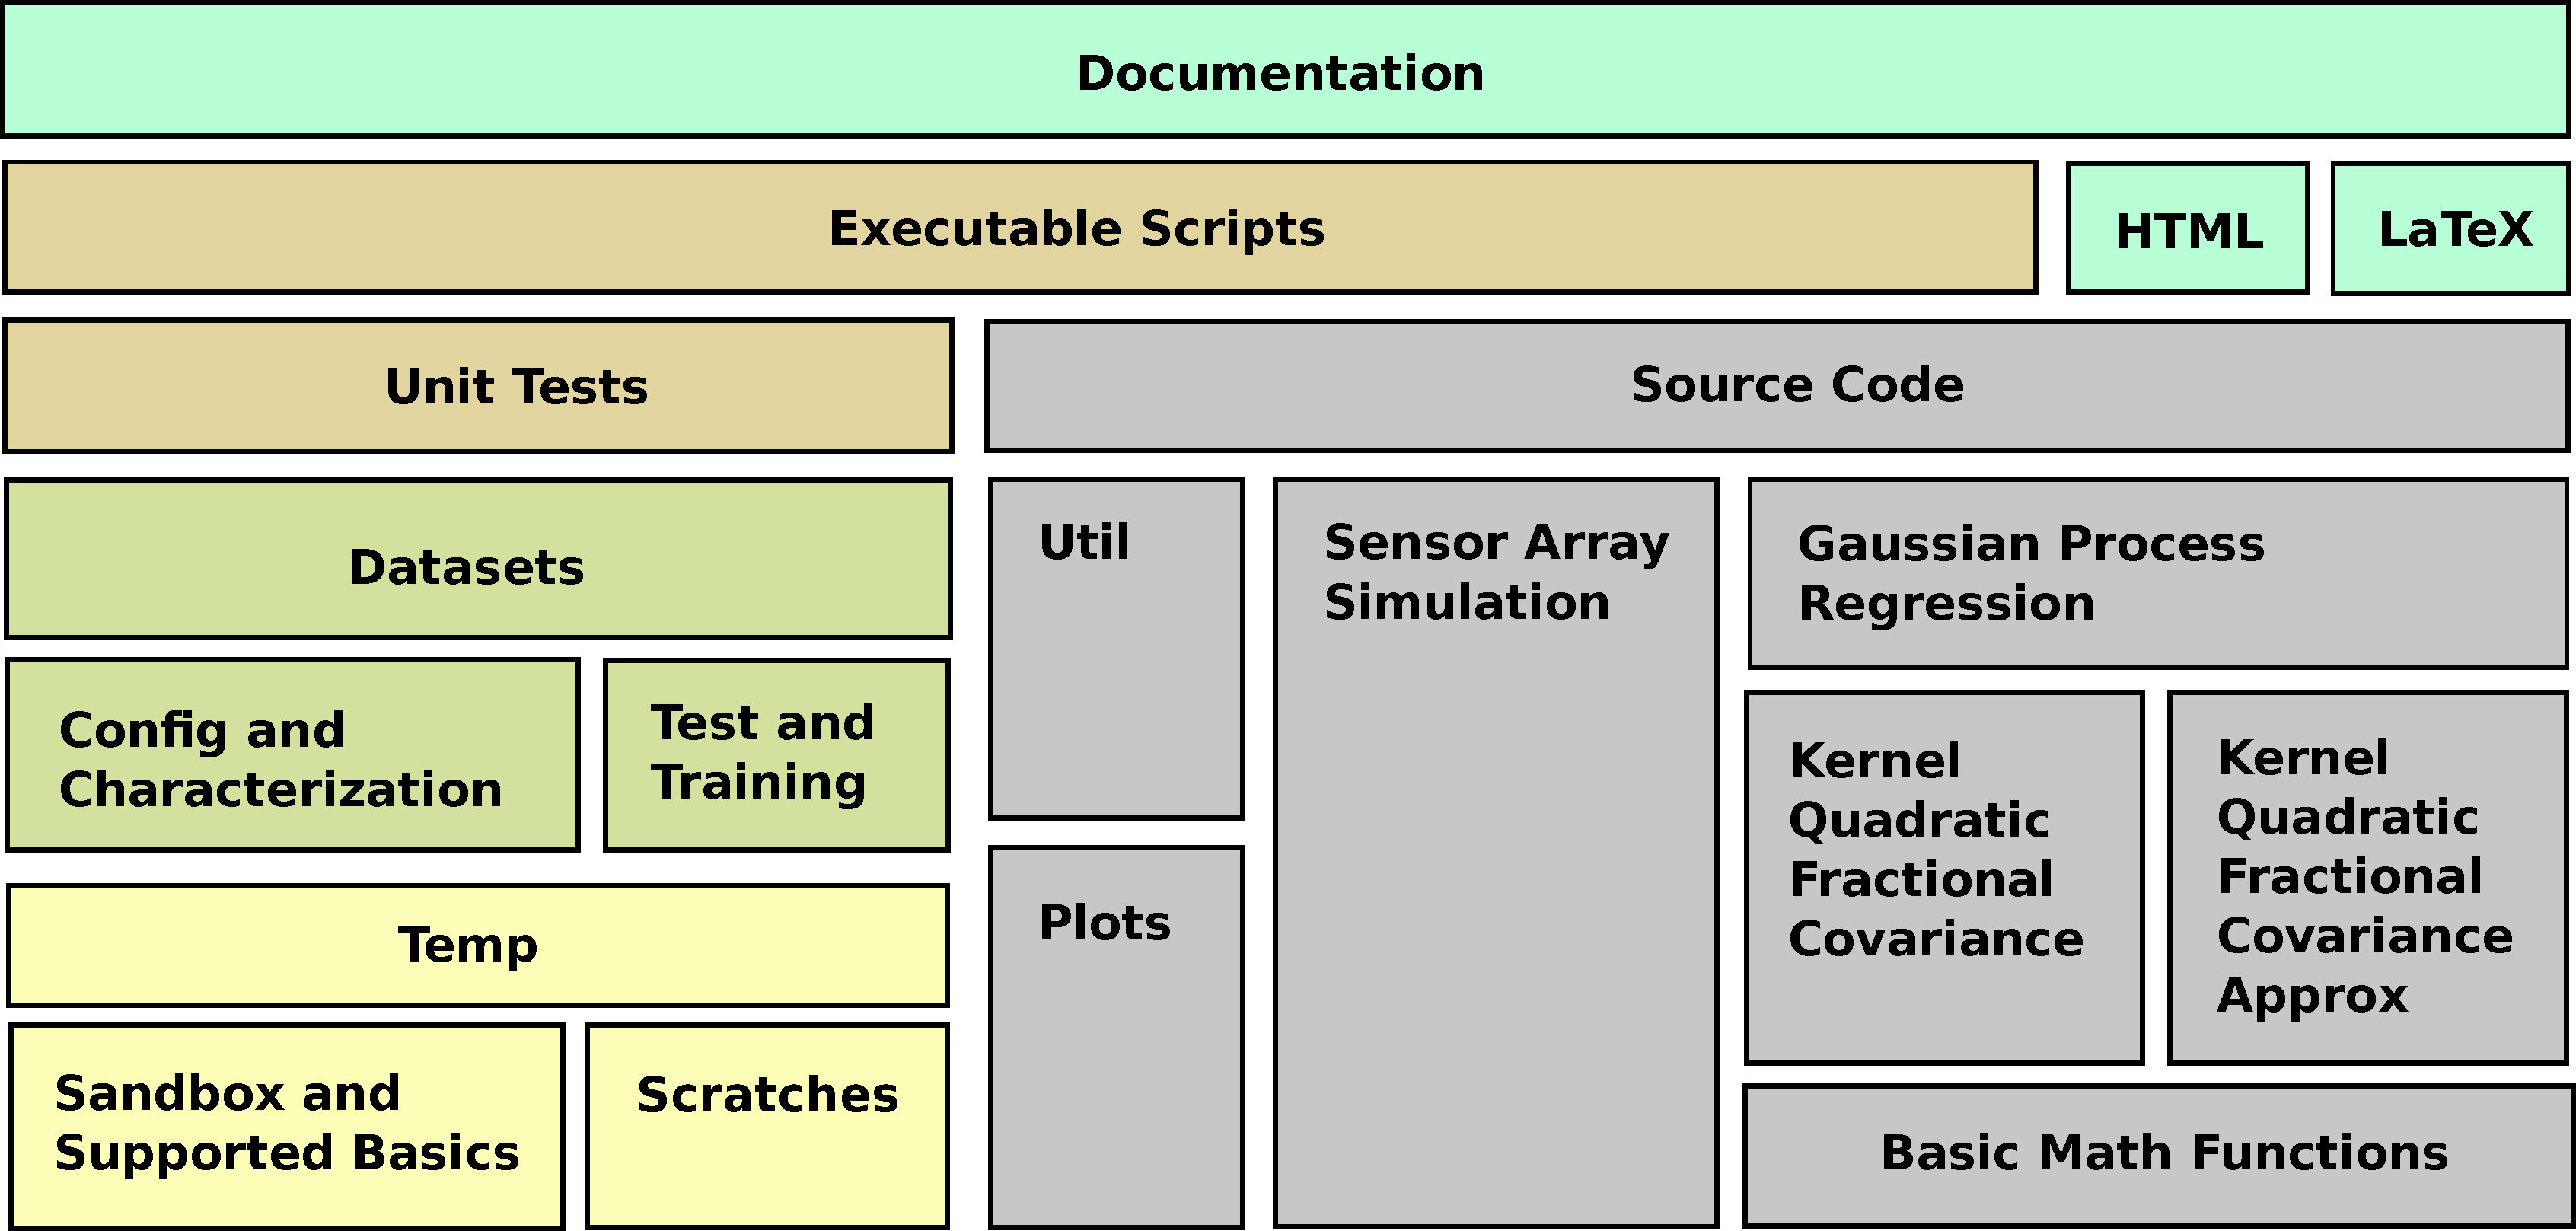
\includegraphics[width=\linewidth]{chapters/images/3-SW-E-OExp/Blockschema_Software}
	\caption[Blockschema Simulations-Software]{Blockschema Simulations-Software}
	\label{fig:blockschemasoftware}
\end{figure}



\clearpage

\subsection{Sensor-Array-Simulation}\label{sub:sensor-array-av}
	\begin{itemize}
		\item Zuordnung Datengenerierung
		\item Nutzung von vorarbeiten
		\item Darstellung des Modul-Funktionsablaufdiagramm
		\item Darstellung des Algorithmus für die Simulation mehrere Positionen
		\item Nutzung des Moduls für eingestellte Konfigurierung
	\end{itemize}

\begin{figure}[tbph]
	\centering
	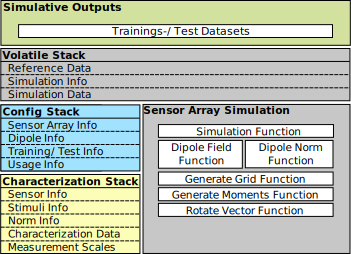
\includegraphics[width=0.7\linewidth]{chapters/images/3-SW-E-OExp/Blockschema_Sensor-Array}
	\caption[Blockschema Sensor-Array-Simulation]{Blockschema Sensor-Array-Simulation}
	\label{fig:blockschemasensor-array}
\end{figure}


\clearpage


\subsection{Gauß-Prozess-Regression}\label{sub:gpr-av}
	\begin{itemize}
		\item Zuordnung Datenanalyse
		\item Nutzung von Vorarbeiten
		\item Darstellung des Modul-Funktionsablaufdiagramm
		\item Aufbau der Modell-Engine und Schnittstellen für neue Kovarianzfunktionen
		\item Darstellung der einzelnen Optimierungsverfahren und Aufzeigen der Unterschiede im vorgehen
 		\item Nutzung des Moduls für eingestellte Konfigurierung
	\end{itemize}


\begin{figure}[tbph]
	\centering
	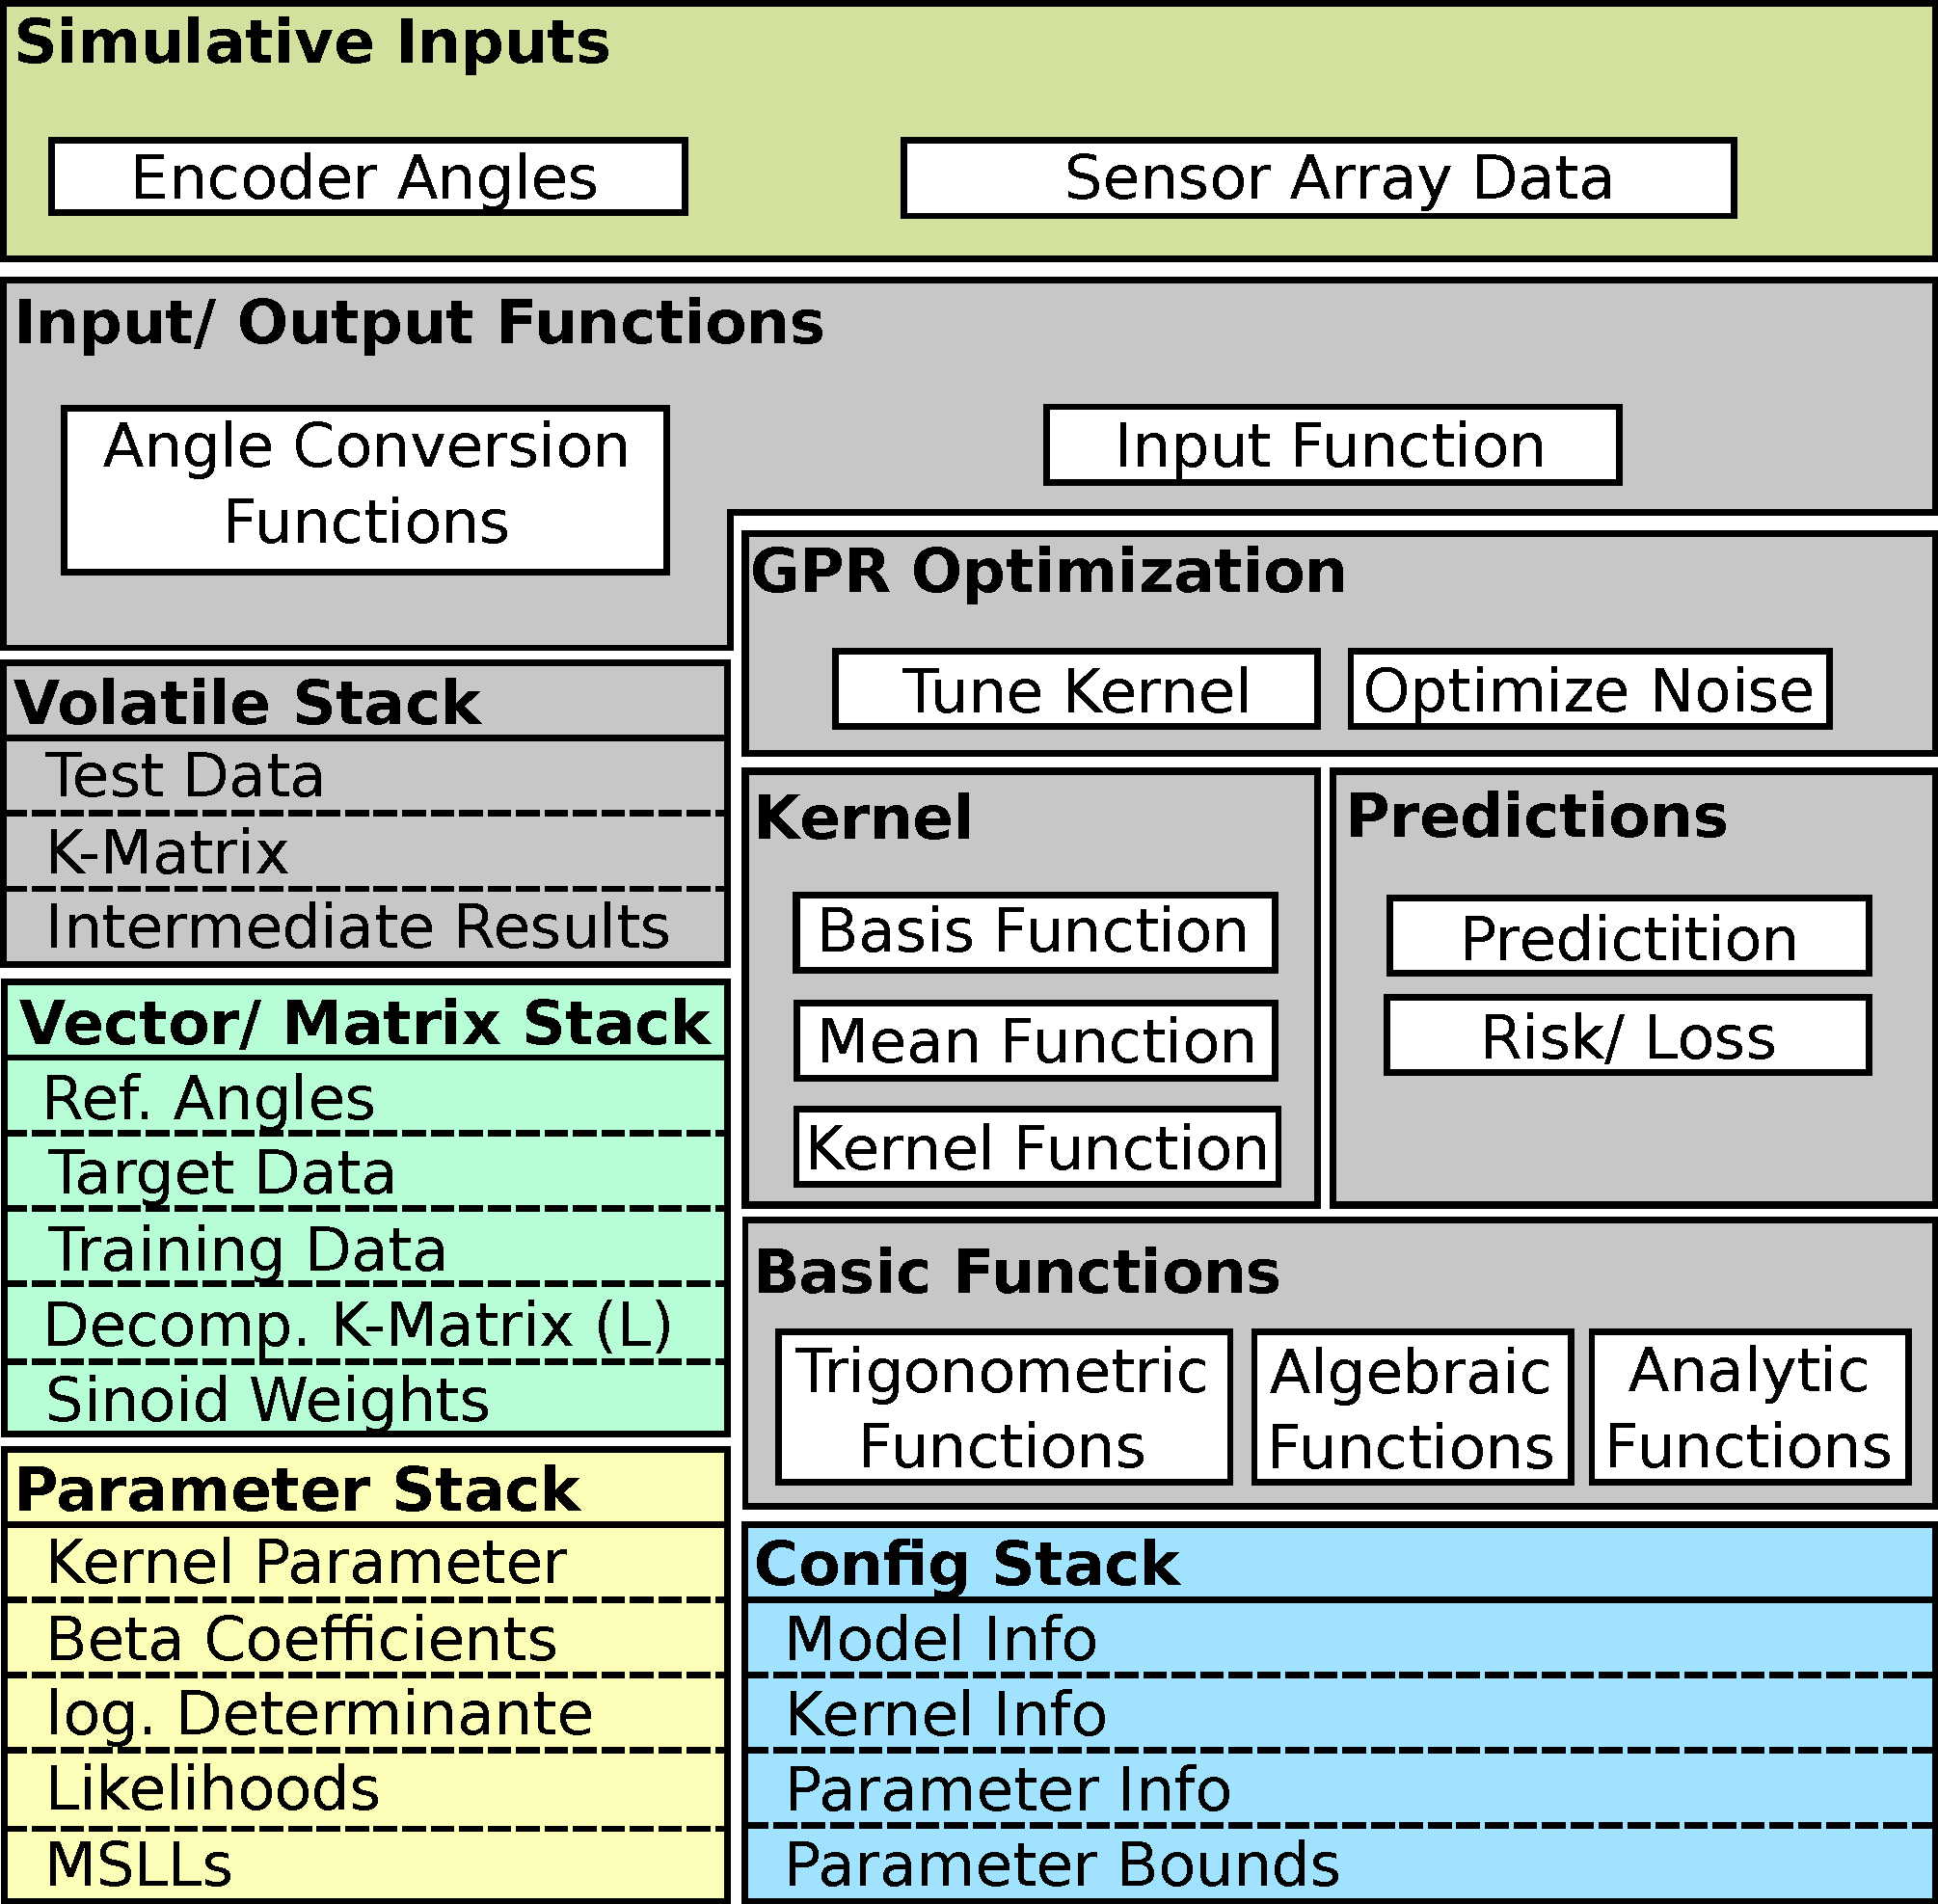
\includegraphics[width=0.7\linewidth]{chapters/images/3-SW-E-OExp/Blockschema_Trainingsphase}
	\caption[Blockschema Trainingsphase Regression]{Blockschema Trainingsphase Regression}
	\label{fig:blockschematrainingsphase}
\end{figure}

\begin{figure}[tbph]
	\centering
	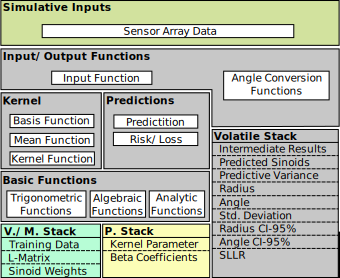
\includegraphics[width=0.7\linewidth]{chapters/images/3-SW-E-OExp/Blockschema_Workphase}
	\caption[Blockschema Arbeitsphase Regression]{Blockschema Arbeitsphase Regression}
	\label{fig:blockschemaworkphase}
\end{figure}


\clearpage


\section{Simulationsprozesse}\label{sec:sim-pro}


\subsection{Sensor-Array-Simulation}\label{sub:sensor-array-pro}


\begin{figure}[tbph]
	\centering
	\includegraphics[width=\linewidth]{chapters/images/3-SW-E-OExp/Sensor-Array-Simulation}
	\caption[Sensor-Array-Simulation Prozessansicht]{Sensor-Array-Simulation Prozessansicht}
	\label{fig:sensor-array-simulation}
\end{figure}

\clearpage

\subsection{Gauß-Prozess-Regression}\label{sub:gpr-pro}


\begin{figure}[tbph]
	\centering
	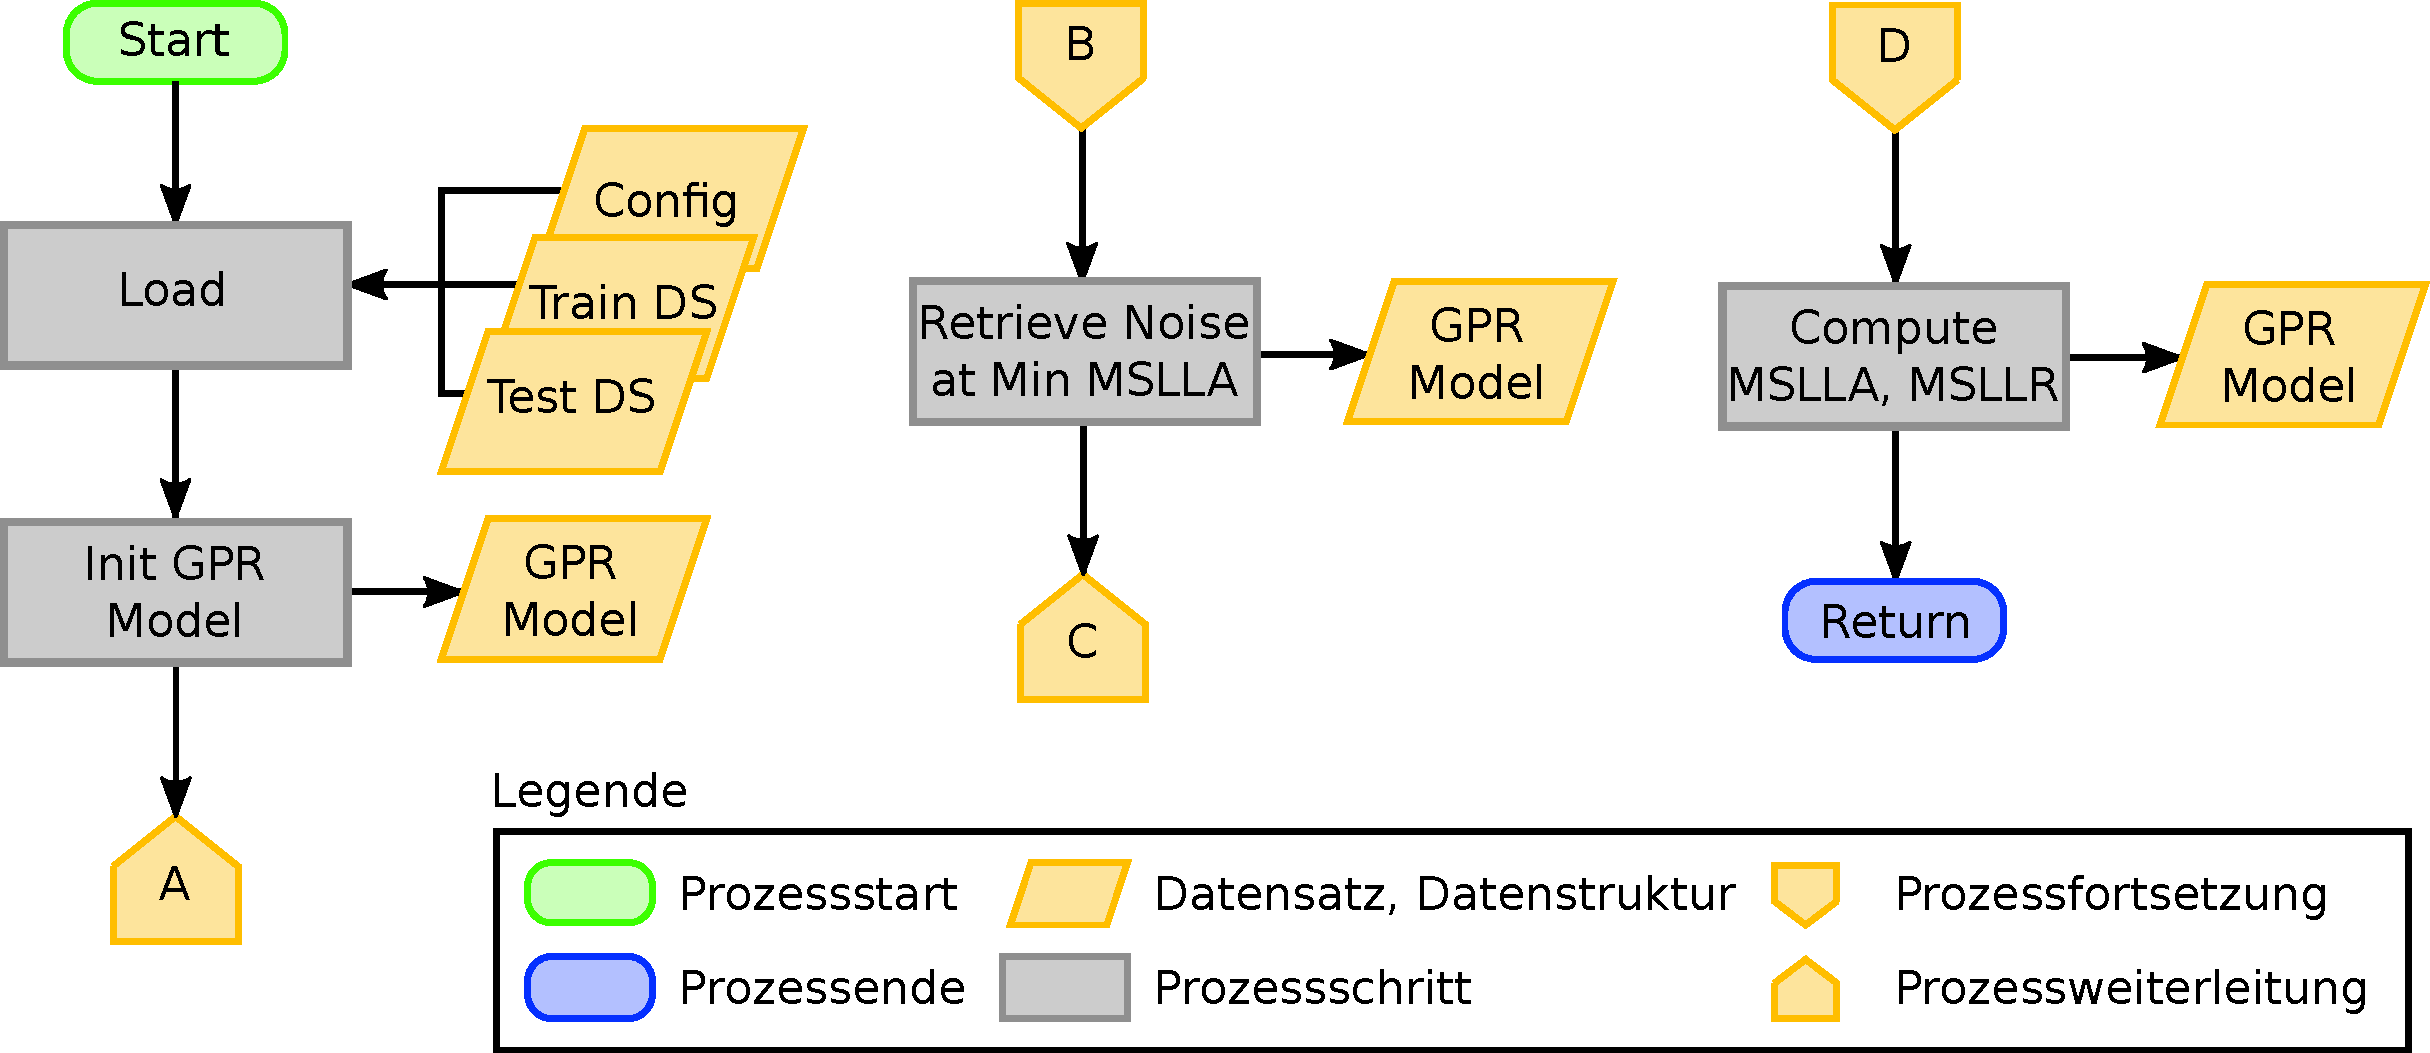
\includegraphics[width=.8\linewidth]{chapters/images/3-SW-E-OExp/GPR_Optimization}
	\caption[Regressionsoptimierung/ -Generalisierung Prozessansicht]{Regressionsoptimierung/ -Generalisierung Prozessansicht}
	\label{fig:gproptimization}
\end{figure}


\begin{figure}[htbp]
	\centering
	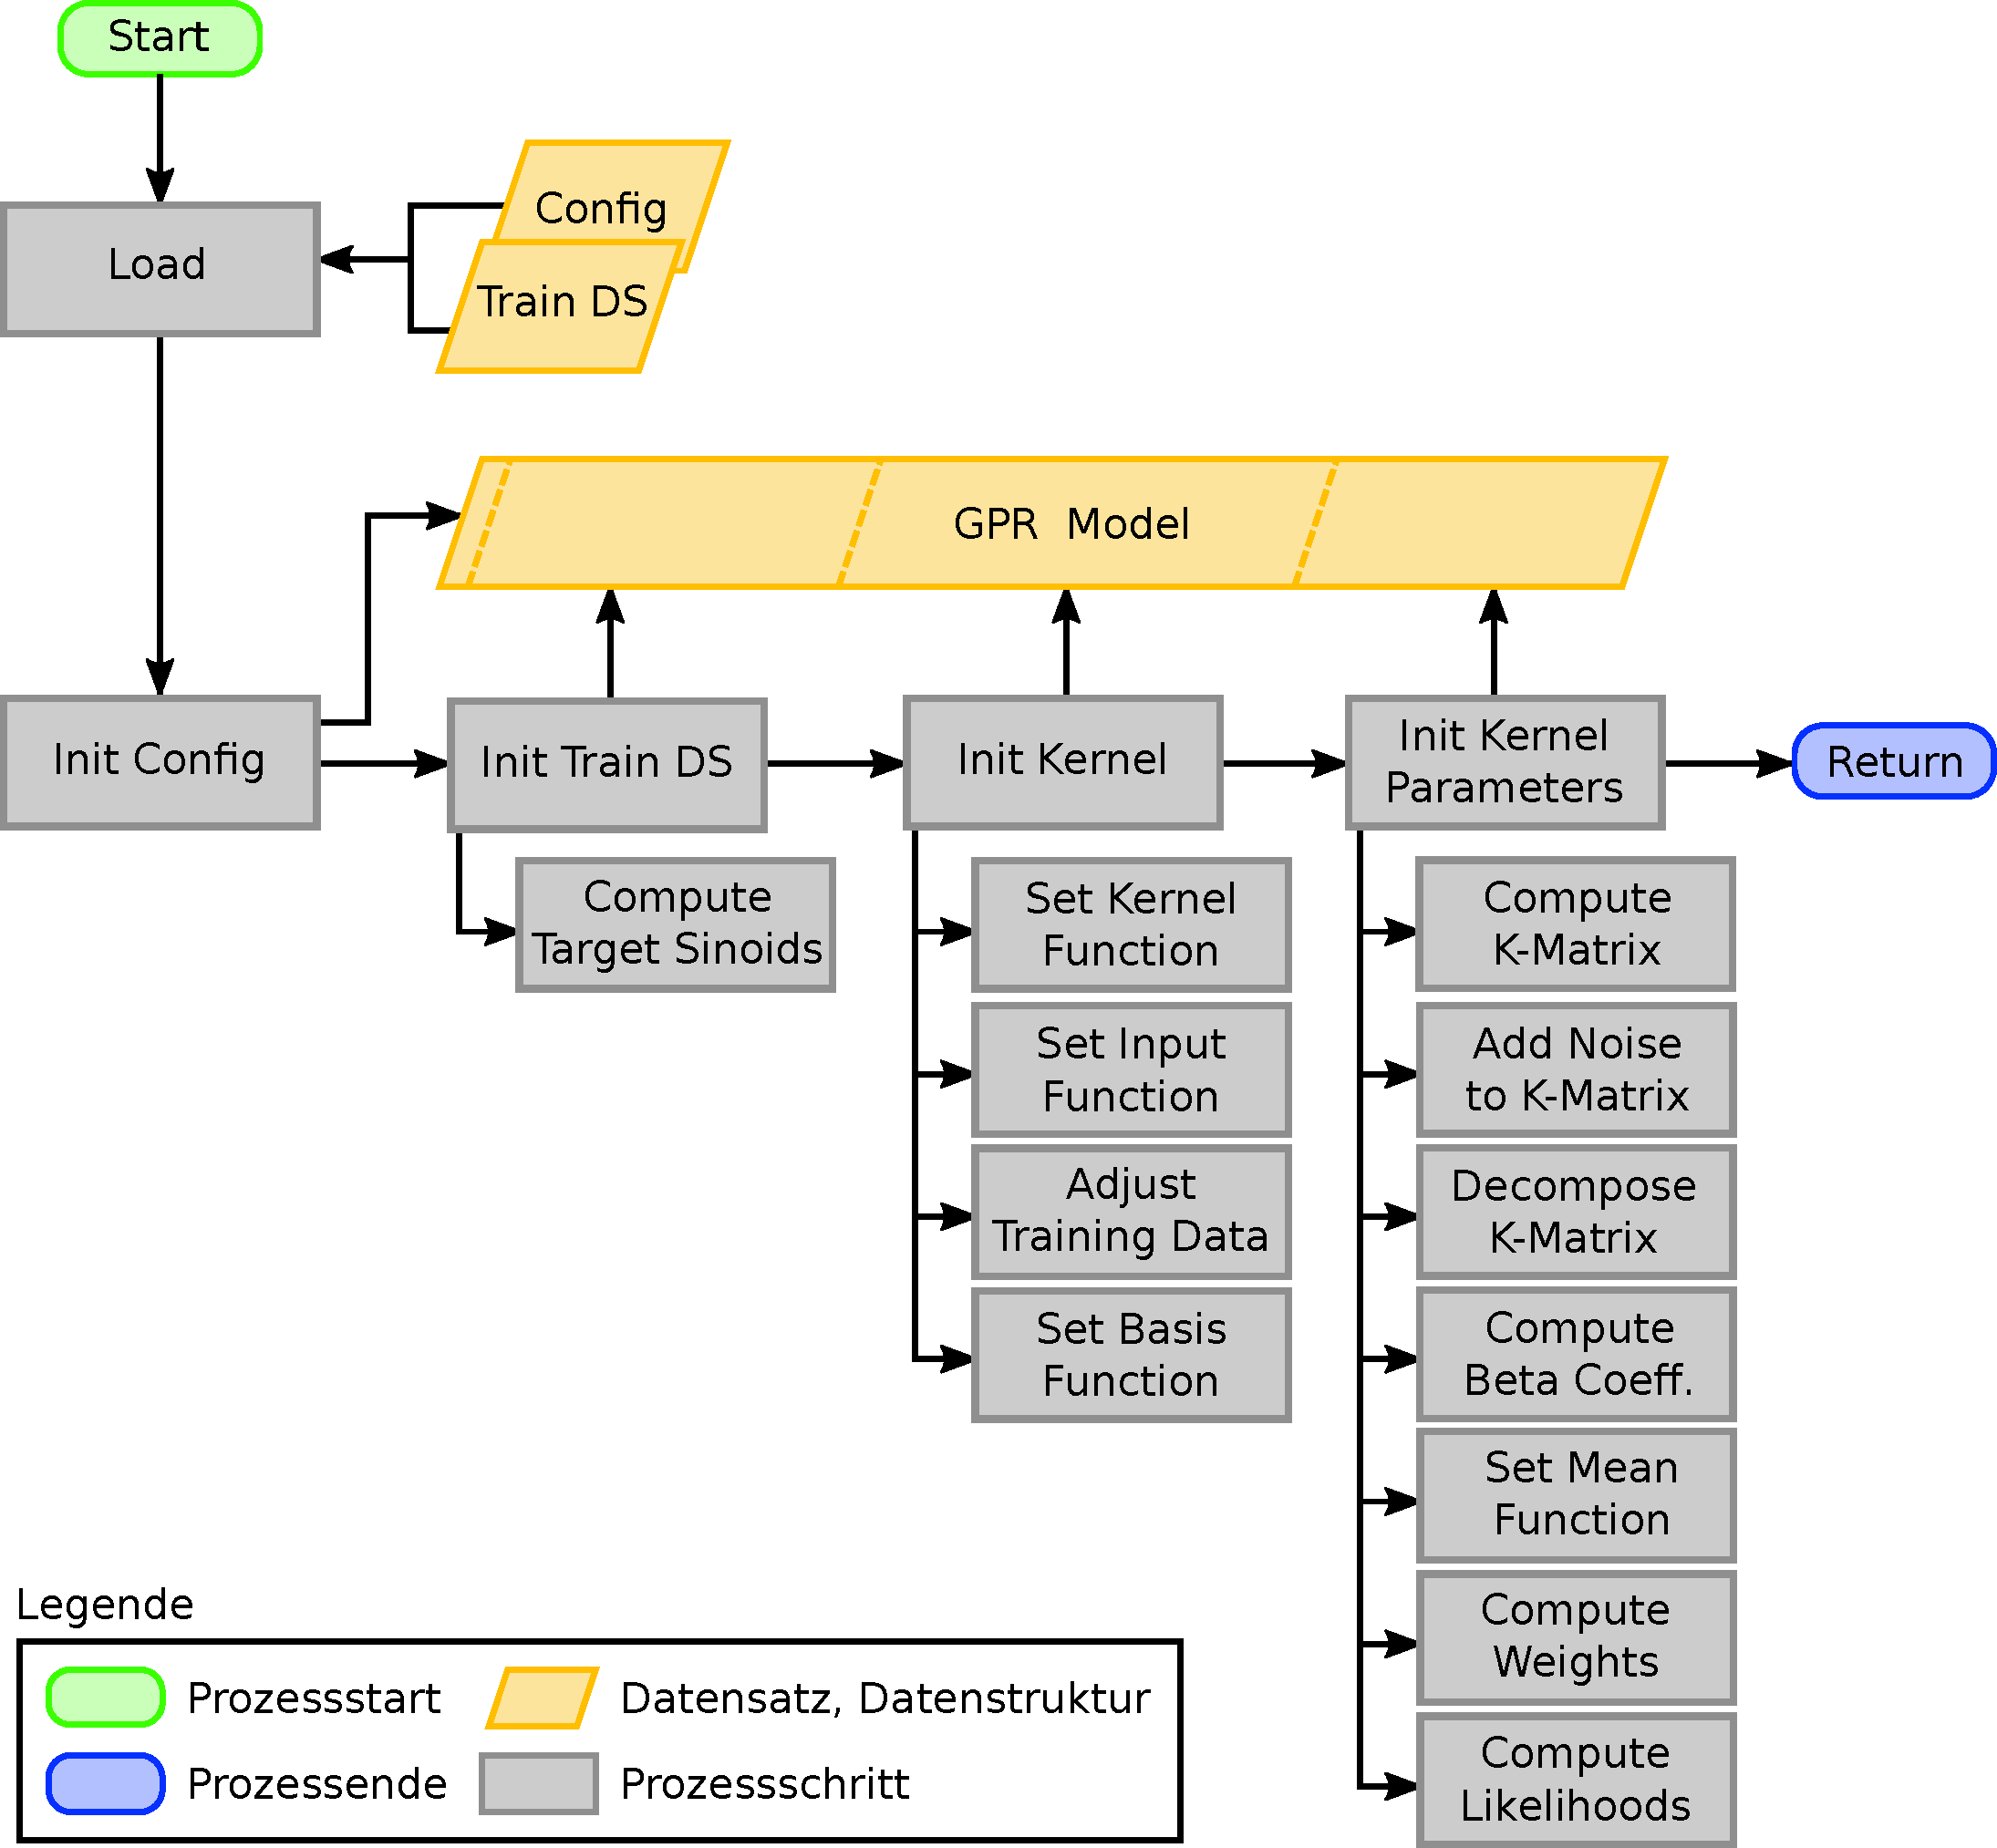
\includegraphics[width=0.7\linewidth]{chapters/images/3-SW-E-OExp/GPR_Initialization}
	\caption[Regressionsinitialisierung Prozessansicht]{Regressionsinitialisierung Prozessansicht}
	\label{fig:gprinitialization}
\end{figure}


\begin{figure}[tbph]
	\centering
	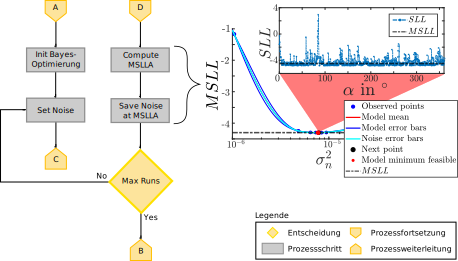
\includegraphics[width=0.85\linewidth]{chapters/images/3-SW-E-OExp/Noise_Optimization}
	\caption[Rauschniveauoptimierung Prozessansicht]{Rauschniveauoptimierung Prozessansicht}
	\label{fig:noiseoptimization}
\end{figure}


\begin{figure}[tbph]
	\centering
	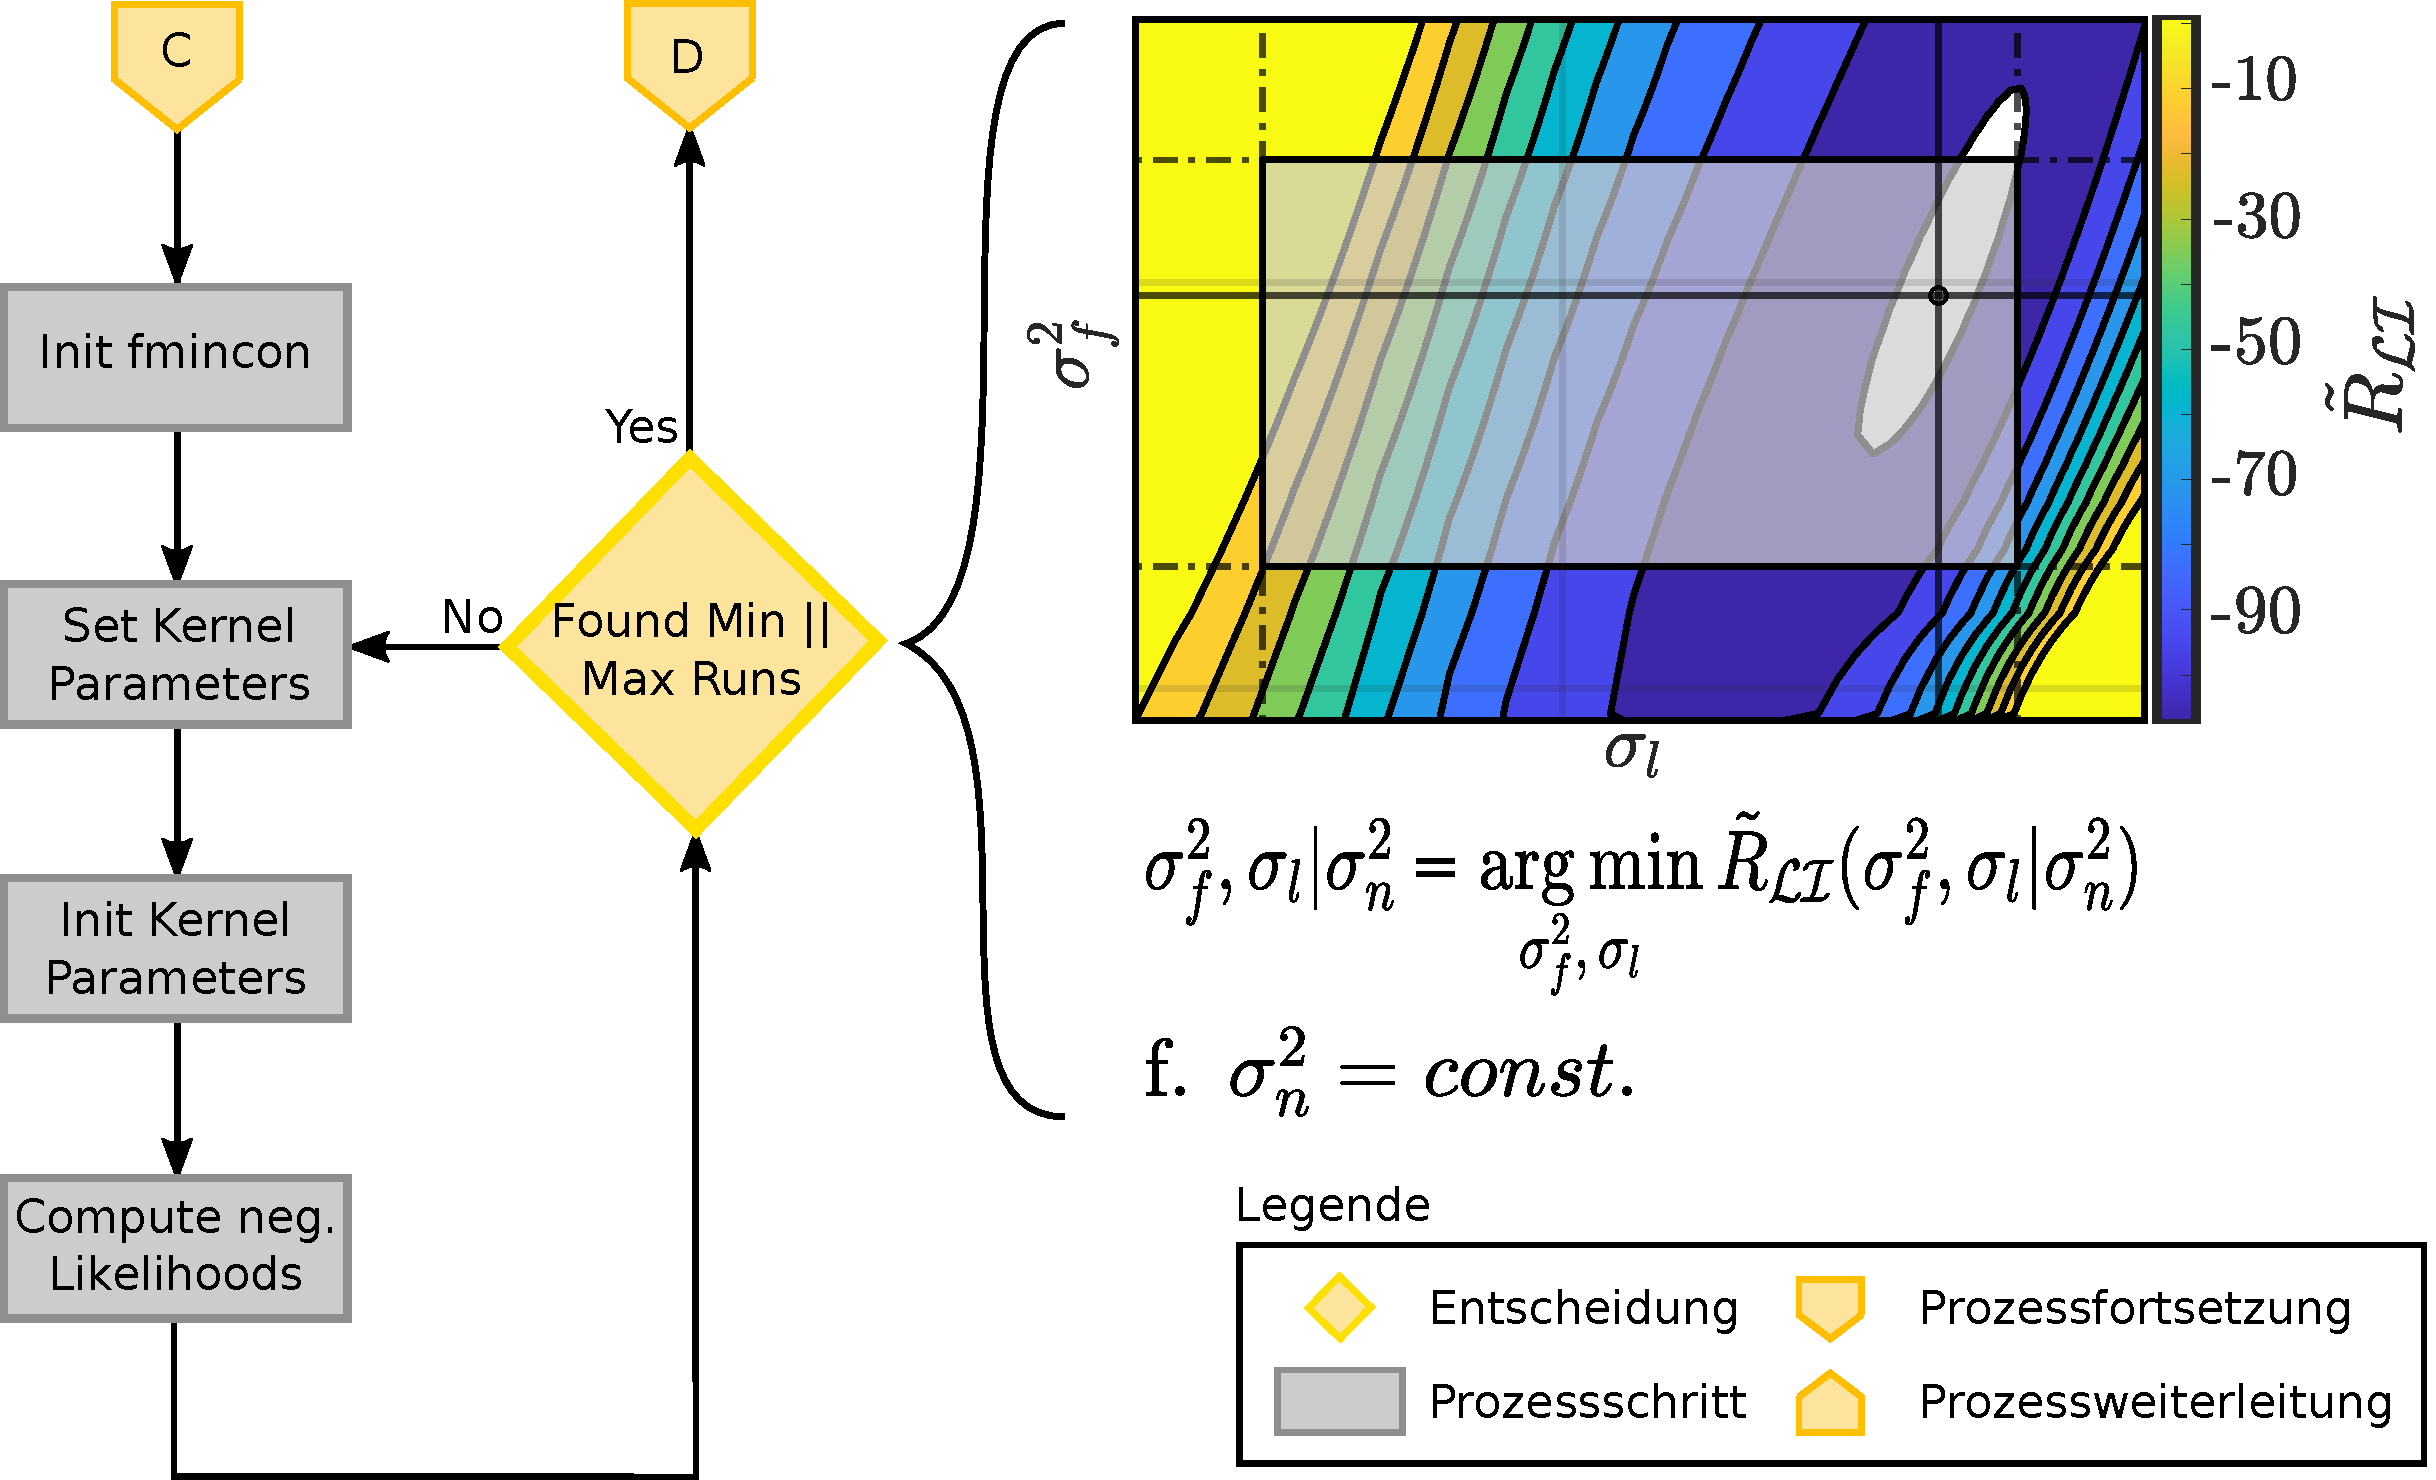
\includegraphics[width=0.8\linewidth]{chapters/images/3-SW-E-OExp/Kernel_Tuning}
	\caption[Regressionsparameteroptimierung Prozessansicht]{Regressionsparameteroptimierung Prozessansicht}
	\label{fig:kerneltuning}
\end{figure}

\clearpage